\documentclass[../BimodalReference.tex]{subfiles}
\begin{document}

\section{Introduction}

The bimodal logic \textbf{TM} combines S5 historical modal operators for necessity ($\nec$) and possibility ($\poss$) with linear temporal operators for past ($\allpast$) and future ($\allfuture$).
Implementing \textbf{TM} in Lean 4 provides a positive RL signal for training AI systems to conduct verified reasoning about past and future contingency in an interpreted formal language.

The semantics is based on \emph{task frames}, which extend Kripke frames with temporal structure.
A task frame consists of world states connected by a \emph{task relation} indexed by temporal durations.
Convex histories are temporal slices through a task frame, representing the possible evolution of a system; the total ones are the possible worlds.

\begin{center}
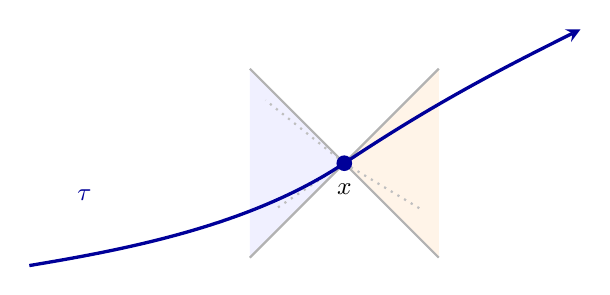
\begin{tikzpicture}[
  worldline/.style={very thick, blue!60!black},
  lightcone fill/.style={opacity=0.15},
  lightcone edge/.style={gray!60, thick},
  counterfactual/.style={dotted, thick, gray!50},
  point/.style={circle, fill=blue!60!black, inner sep=2pt}
]
  % Define the marked point P (x) at the inflection of the single S-curve
  % The worldline passes through P with one continuous up-right tangent
  \coordinate (P) at (0.5,-0.2);

  % Light cones are drawn axis-aligned (conventional), independent of the
  % worldline tangent. Light cone size: 1.2 units (2/3 of original)

  % Future light cone (opens right, horizontal tangent = 0 degrees)
  \begin{scope}[shift={(P)}]
    \fill[orange!60, lightcone fill] (0,0) -- (1.2,1.2) -- (1.2,-1.2) -- cycle;
    \draw[lightcone edge] (0,0) -- (1.2,1.2);
    \draw[lightcone edge] (0,0) -- (1.2,-1.2);
  \end{scope}

  % Past light cone (opens left, 180 degrees)
  \begin{scope}[shift={(P)}]
    \fill[blue!40, lightcone fill] (0,0) -- (-1.2,1.2) -- (-1.2,-1.2) -- cycle;
    \draw[lightcone edge] (0,0) -- (-1.2,1.2);
    \draw[lightcone edge] (0,0) -- (-1.2,-1.2);
  \end{scope}

  % Draw counterfactual paths within cones
  % Past paths (within past cone, heading left)
  \draw[counterfactual] (P) -- (-0.5,0.6);
  \draw[counterfactual] (P) -- (-0.4,-0.8);

  % Future paths (within future cone, heading right)
  \draw[counterfactual] (P) -- (1.6,0.5);
  \draw[counterfactual] (P) -- (1.5,-0.8);

  % Draw the S-shaped main worldline (actual history) as ONE smooth S:
  % left half concave-up, right half concave-down, sharing a single sloped
  % tangent (slope ~0.67) through P so x is the sole inflection point.
  \draw[worldline, ->, >=stealth] (-3.5,-1.5)
    .. controls (-2.3,-1.3) and (-0.7,-1.0) .. (P)
    .. controls (1.7,0.6) and (2.6,1.05) .. (3.5,1.5);

  % Label tau above the worldline near its beginning
  \node[font=\small, blue!60!black] at (-2.8,-0.6) {$\tau$};

  % Draw the marked point P on top
  \node[point] at (P) {};
  \node[below=4pt, font=\small] at (P) {$x$};

\end{tikzpicture}
\end{center}

\noindent
The diagram above illustrates the conceptual structure underlying TM logic.
The solid curve $\tau$ represents a single possible world---a temporal sequence of states.
From any point $x$ along a history, the past and future light cones contain all states that are modally accessible.
The necessity operator $\nec$ quantifies over all possible histories, though we may often restrict to those histories that pass through the world state $\tau(x)$.
The temporal operators $\allpast$ and $\allfuture$ quantify over past and future times which, given a particular history, determines the range of past and future world states that history occupies relative to a given time.
These primitive operators may then be used to define a host of combined operators of interest.

\subsection*{Project Structure}

The Lean 4 implementation is in the \texttt{Bimodal/} directory:
\begin{itemize}
  \item \texttt{Syntax/} -- Defines the formula language with 6 primitive constructors and derived operators.
  \textbf{Complete.}
  \item \texttt{ProofSystem/} -- Axioms (14 schemata) and inference rules (7 rules) forming a Hilbert-style proof system.
  \textbf{Complete.}
  \item \texttt{Semantics/} -- Task frames model possible worlds; histories model time; truth conditions define meaning.
  \textbf{Complete.}
  \item \texttt{Metalogic/} -- Soundness theorem (proven: all axioms valid, rules preserve validity), deduction theorem (proven: enables assumption introduction), completeness via the semantic canonical model (Lindenbaum lemma proven, truth lemma proven, weak completeness proven), and decidability via tableau-based decision procedure (soundness and completeness proven).
  \textbf{Complete.}
  \item \texttt{Theorems/} -- Perpetuity principles and modal theorems derived from the axiom system.
  \textbf{Partial.}
\end{itemize}

\end{document}
